\begin{figure*}
  \centering
    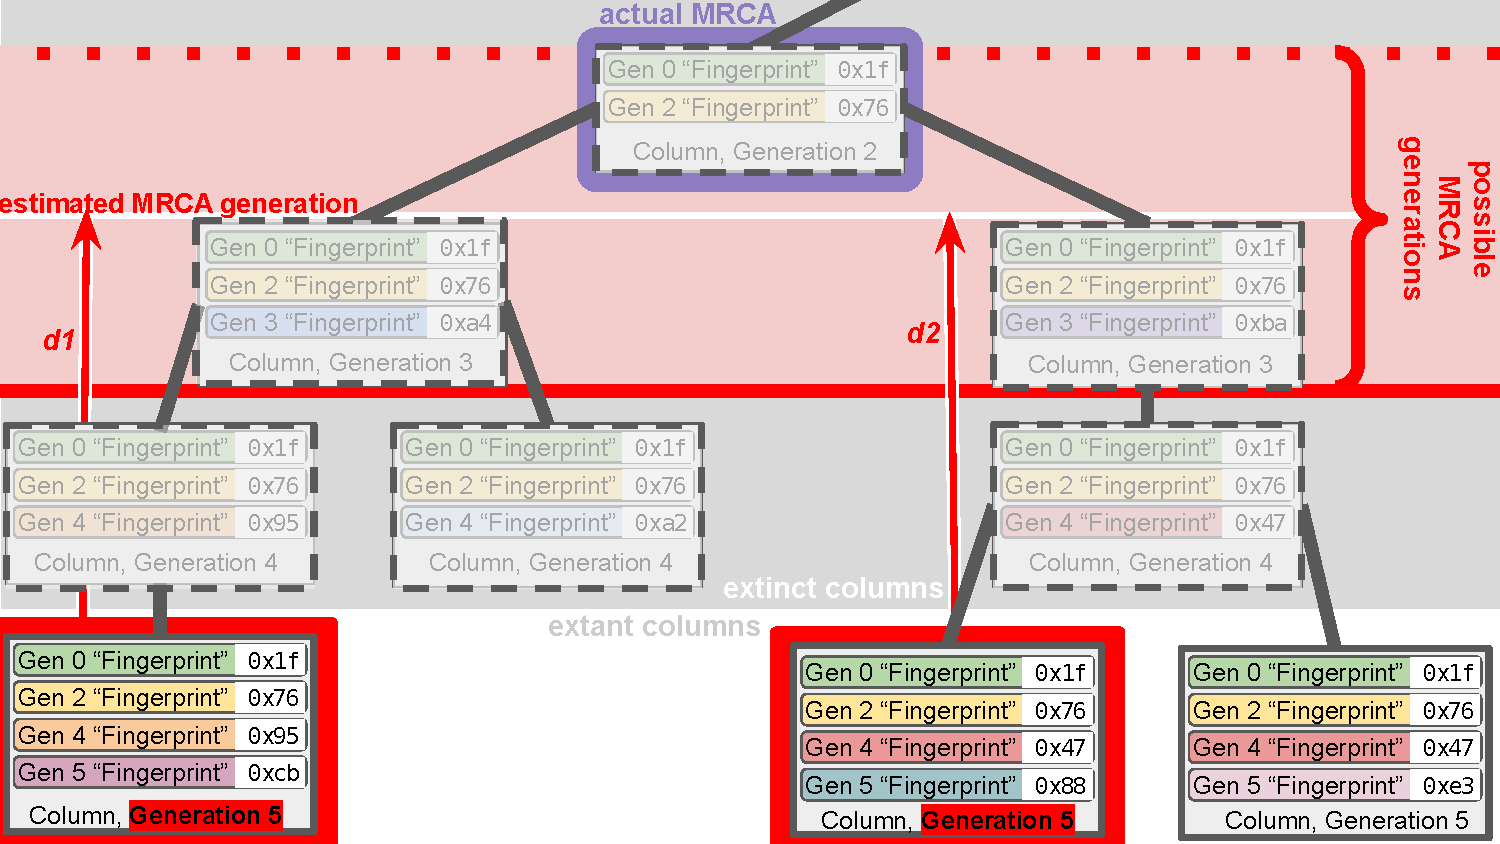
\includegraphics[width=\textwidth]{img/phylogenetic-inference}
    \caption{
    Cartoon illustration of column inheritance along a phylogenetic tree and the process to infer phylogenetic history along extant columns.
    This scenario supposes a stratum retention policy where only strata from even generations are retained.
    The common ancestor of the focal clade, which is at generation 2, is shown at top.
    Generation 3 columns inherit that ancestor's strata and each append a new stratum.
    Generation 4 columns append another new stratum then eliminate their generation 3 strata.
    Finally, another generation elapses to yield generation 5 strata.
    Suppose that only generation 5 strata are extant.
    So, greyed-out columns above are not directly observable.
    Phylogenetic history is deduced by pairwise comparison between extant columns.
    For each pair (like the example highlighted in red) a phylogenetic distance can be computed as the sum generations elapsed to each extant column after the estimated generation of their MRCA.
    These pairwise distances can then be fed into a phylogeny reconstruction algorithm.
    }
  \label{fig:phylogenetic-inference}
\end{figure*}
